\documentclass[12pt]{article}
\usepackage{helvet}
\usepackage{graphicx}
\usepackage{geometry}
\geometry{
    a4paper,
    top = 2cm,
    left = 2cm,
    right = 2cm,
    bottom = 3cm
}
\usepackage[utf8]{inputenc}
\usepackage[spanish,mexico]{babel} % Renombra en automático los elementos a español
\addto\captionsspanish{
  \renewcommand{\figurename}{Imagen}
  \renewcommand{\tablename}{Tabla}
}
\usepackage{float}  % Etiqueta 'H' (mayus) en figuras (imágenes)
\usepackage{array}  % Padding en tablas
\usepackage{tabularx}
\usepackage{url}    % Etiqueta url en .bib
\usepackage{booktabs}   % Manejo de caudros (tablas)
\usepackage[T1]{fontenc}    % Codificación de fuentes
\usepackage[autostyle, spanish=mexican]{csquotes}       % Paquete para comillas tipográficas
\usepackage{comment}    % Comentar bloques de líneas mediante begin-end
\usepackage{multicol}   % Para poner contenido a doble columna
\usepackage{enumitem}   % Para utilizar [noitemsep, topsep=0pt] en itemize
\usepackage{amsmath}
\usepackage{mathabx} % Para testar en math mode
\usepackage{comment}
\usepackage{longtable}
\usepackage[hidelinks]{hyperref}
\usepackage{caption}
\usepackage[
  backend=biber,
  style=apa,
  sorting=nyt
]{biblatex}
\DeclareLanguageMapping{spanish}{spanish-apa}
\renewcommand{\familydefault}{\sfdefault}
\newenvironment{localsubgroup}
  {$\left\{\tabular{l}}
  {\endtabular\right.$}


\addbibresource{bibliography/t02.bib}

\begin{comment}
INDICACIONES DEL PROFESOR:
Fecha de entrega: 12 de septiembre de 2026
Título: Memoria y procesos
Número: 2
Tipo: Tarea

Instrucciones del profesor:

a) Investigar conceptos de memorias
- Definición de memoria
- Clasificación de memoria
- Tipos de memoria
- Evolución de memoria RAM - Año, nombre e imagen
- Evolución de memoria secundaria (Almacenamiento) - Año, nombre e imagen

b) ¿Qué entiendes por memoria de intercambio? ¿Cuál es la función que realiza en los Sistemas Operativos?

c) Investigar:
- ¿Qué es un proceso?
- ¿Qué es un hilo de ejecución?
- La diferencia entre hilos y procesos.
- Características de los procesos.

Un máximo de 25 hojas.

RESTRICCIÓN DE EXTENSIÓN:
Régimen normativo del repositorio (18 a 40 páginas, objetivo 27), estrictamente acotado por la indicación del profesor a un máximo de 25 hojas. Presupuesto meta: entre 23 y 25 páginas totales (portada, índice, desarrollo, conclusiones y referencias).

ÍNDICE PROPUESTO:
1. Fundamentos y taxonomía de la memoria en los sistemas de cómputo [~3.5 págs.]
   1.1 Definición formal y rol en la arquitectura de von Neumann [~1.0 pág.]
   1.2 Jerarquía de memoria y principios de localidad [~1.0 pág.]
   1.3 Criterios de clasificación y tipos de memoria [~1.5 págs.]
2. Evolución histórica de la memoria principal y tecnologías RAM [~4.5 págs.]
   2.1 Hitos pioneros del almacenamiento primario [~1.5 págs.]
   2.2 Memorias de acceso aleatorio estáticas y dinámicas (SRAM vs. DRAM) [~1.0 pág.]
   2.3 Evolución de las tecnologías DRAM sincrónicas y de alta tasa de transferencia [~2.0 págs.]
3. Evolución histórica de la memoria secundaria y almacenamiento masivo [~4.5 págs.]
   3.1 Tecnologías electromecánicas y magnéticas tempranas [~1.5 págs.]
   3.2 Medios ópticos y consolidación de discos duros magnéticos (HDD) [~1.0 pág.]
   3.3 Tecnologías de estado sólido y almacenamiento no volátil avanzado [~2.0 págs.]
4. Memoria de intercambio (Swapping) y gestión de memoria virtual [~3.0 págs.]
   4.1 Definición y distinción técnica: intercambio de procesos vs. paginación bajo demanda [~1.0 pág.]
   4.2 Funciones y operatividad de la memoria de intercambio en el sistema operativo [~1.0 pág.]
   4.3 Rendimiento, degradación por hiperpaginación (Thrashing) y mitigación [~1.0 pág.]
5. Arquitectura y ciclo de vida de los procesos [~3.0 págs.]
   5.1 Definición formal de proceso y organización en memoria [~1.0 pág.]
   5.2 Estructura y características del proceso: Bloque de Control de Proceso (PCB) [~1.0 pág.]
   5.3 Modelo de estados y transiciones en la ejecución del proceso [~1.0 pág.]
6. Hilos de ejecución y análisis comparativo frente a procesos [~3.5 págs.]
   6.1 Definición formal de hilo (Thread) y estructura de control (TCB) [~1.0 pág.]
   6.2 Modelos de gestión de hilos y correspondencia de planificación [~1.0 pág.]
   6.3 Estudio comparativo y diferencial entre procesos e hilos [~1.5 págs.]
7. Conclusiones personales [~2.0 págs.]
Referencias [~1.0 pág.]
\end{comment}

\begin{document}
\pagenumbering{roman}

\begin{titlepage}
  \thispagestyle{empty}
  \newgeometry{left = 1cm, right = 1cm, top = 1cm, bottom = 2cm}

  \noindent
  \begin{minipage}[c]{3.5cm}
    
\includegraphics[width=3.5cm]{media/titlepage/Escudo-UNAM.pdf}
  \end{minipage}\hfill
  \begin{minipage}[c][3.5cm][c]{\dimexpr\textwidth-7cm\relax}
    \centering
    {\large\textbf{Universidad Nacional Autónoma de México}\\[0.6em] 
    \Large\textbf{Facultad de Ingeniería}\\[0.6em]
    \large Sistemas Operativos}
  \end{minipage}\hfill
  \begin{minipage}[c]{3.5cm}
    \raggedleft
    
\includegraphics[width=3.5cm]{media/titlepage/FI.png}
  \end{minipage}
\centering\huge
  \vfill
    Grupo 1 \\
    Ing. Angel Isidro Mercado
  \vfill
    \textbf{Tarea 2. Memoria y procesos}
  \vfill\large
    320304435 - Cabrera Rojas Oscar
  \vfill

  \noindent\footnotesize \hfill Ciudad Universitaria, CDMX a 12 de septiembre del 2026
\end{titlepage}
\restoregeometry

\tableofcontents

\newpage
\pagenumbering{arabic}
\setcounter{page}{1}

\section{Fundamentos y taxonomía de la memoria en los sistemas de cómputo}
\label{sec:fundamentosTaxonomiaMemoria}

\subsection{Definición formal y rol en la arquitectura de von Neumann}
\label{sec:definicionArquitecturaVonNeumann}

En la teoría de sistemas computacionales y la ingeniería de computadores, la memoria no constituye un mero repositorio pasivo de información, sino un subsistema funcional activo y estructurado concebido para almacenar estados binarios transitorios o permanentes organizados en celdas direccionables numéricamente \parencite[\S 1.1, p.\ 31]{stallings2018operating}. Desde la formulación seminal del modelo de John von Neumann en 1945, la memoria principal ocupa el núcleo operativo del procesamiento automático de datos mediante el principio de programa almacenado (\textit{stored-program concept}). Bajo este paradigma, las instrucciones de control del programa y los datos sobre los cuales operan dichas instrucciones residen indistintamente en el mismo medio físico de almacenamiento y comparten un espacio de direccionamiento lineal homogéneo \parencite[\S 1.2, p.\ 8]{silberschatz2006fundamentos}.

La interacción entre la unidad central de procesamiento (CPU) y la memoria opera mediante registros dedicados y buses del sistema. La CPU gobierna los accesos con el registro de direcciones de memoria (\textit{memory address register}, MAR), que fija la coordenada numérica de la celda, y el registro de búfer o datos (\textit{memory buffer register}, MBR), que sostiene temporalmente la palabra transferida \parencite[\S 1.1, p.\ 31]{stallings2018operating}. Esta transferencia se realiza a través del bus de direcciones (cuyo ancho fija el espacio direccionable), el bus de datos (ancho de palabra transferible) y el bus de control (señales de temporización y selección de lectura/escritura) \parencite[\S 2.3, p.\ 64]{deitel2004operating}. El procesamiento se rige por el ciclo de instrucción-ejecución (\textit{fetch-decode-execute-store}): el contador de programa (PC) carga la dirección en el MAR para transferir la instrucción al MBR y al registro de instrucción (IR) (\textit{fetch}); la unidad de control decodifica el código de operación (\textit{decode}); la unidad aritmético-lógica (ALU) opera sobre los operandos (\textit{execute}); y los resultados se escriben en memoria o registros (\textit{store}) \parencite[\S 1.2, p.\ 8]{silberschatz2006fundamentos}.

La memoria es agnóstica a la semántica de los datos binarios que aloja. Al unificarse el bus de instrucciones y datos en von Neumann, surge el \enquote{cuello de botella de von Neumann} (\textit{von Neumann bottleneck}) \parencite[\S 2.3, p.\ 64]{deitel2004operating}: como la velocidad de la CPU escaló históricamente más rápido que la latencia de la DRAM, el procesador inserta ciclos de espera (\textit{wait states}) aguardando datos. En contraste, la arquitectura Harvard separa físicamente los buses de instrucciones y datos; aunque más costosa para memoria principal, esta separación se preserva internamente en las cachés de nivel 1 (L1i y L1d), manteniendo una interfaz unificada hacia el exterior \parencite[\S 1.6, p.\ 49]{stallings2018operating}.

\subsection{Jerarquía de memoria y principios de localidad}
\label{sec:jerarquiaMemoriaLocalidad}

El diseño del subsistema de memoria balancea tres restricciones físicas y económicas: capacidad, tiempo de acceso y costo por bit \parencite[\S 1.5, pp.\ 45--46]{stallings2018operating}. A menor tiempo de acceso, mayor es el costo monetario por bit; a mayor capacidad, menor es el costo unitario, pero mayor es la latencia por retardos de decodificación y líneas físicas \parencite[\S 2.3, p.\ 64]{deitel2004operating}. Para compatibilizar velocidad y costo masivo, los sistemas organizan el almacenamiento en una pirámide jerárquica escalonada \parencite[\S 1.5, p.\ 47]{stallings2018operating}. En la cúspide se ubican los registros internos de la CPU (fracciones de ciclo, cientos de bytes). Le sigue la memoria caché multinivel (L1, L2, L3) en tecnología estática (\textit{static random-access memory}, SRAM), con latencias de 2 a 40 ciclos y capacidades de kilobytes a megabytes \parencite[\S 2.3, p.\ 64]{deitel2004operating}. Debajo se posiciona la memoria principal en tecnología dinámica (\textit{dynamic random-access memory}, DRAM), que aloja los procesos activos con latencias de decenas de nanosegundos y capacidades de gigabytes. En la base se sitúa el almacenamiento secundario no volátil (HDD, SSD Flash NAND) y terciario (cintas, ópticos), brindando terabytes a bajo costo con latencias de microsegundos a milisegundos \parencite[\S 1.8, pp.\ 21--23]{silberschatz2006fundamentos}. Esta pirámide se ilustra en la Img.~\ref{fig:jerarquiaMemoriaPiramide}.

\begin{figure}[htbp]
    \centering
    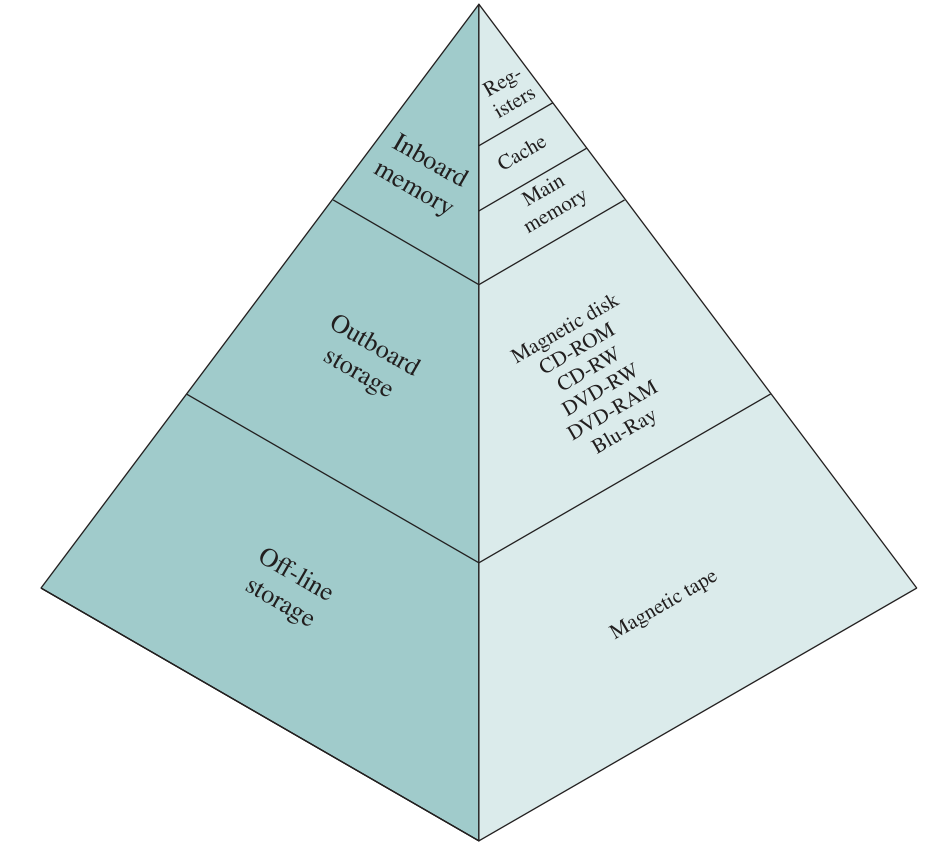
\includegraphics[width=\columnwidth]{media/t02/jerarquiaMemoriaPiramide.png}
    \caption{Niveles jerárquicos de memoria, compensación costo-rendimiento y tiempos de acceso \parencite[\S 1.5, p.\ 47]{stallings2018operating}.}
    \label{fig:jerarquiaMemoriaPiramide}
\end{figure}

La operatividad y viabilidad técnica de esta jerarquía descansa en el principio de localidad de referencia (\textit{locality of reference}), formulado formalmente por Peter J. Denning en 1968 \parencite[\S 1.5, p.\ 48]{stallings2018operating}. Este postulado empírico establece que, durante la ejecución de un programa informático, las referencias a memoria efectuadas por la CPU tienden a agruparse en regiones o bloques sumamente acotados del espacio de direcciones durante intervalos de tiempo determinados. El fenómeno se descompone en dos propiedades fundamentales:
\begin{itemize}[noitemsep, topsep=0pt]
    \item \textbf{Localidad temporal:} Si una posición de memoria concreta es accedida en un instante $t$, existe una probabilidad cuantitativamente elevada de que sea referenciada nuevamente en un instante cercano $t + \Delta t$. Este comportamiento es típico de estructuras de bucles iterativos (\textit{loops}), variables acumuladoras, contadores y subrutinas invocadas con frecuencia en el cuerpo de un algoritmo \parencite[\S 1.5, p.\ 48]{stallings2018operating}.
    \item \textbf{Localidad espacial:} Si una dirección de memoria es referenciada en un instante dado, existe una alta probabilidad de que las posiciones continuas y adyacentes a ella sean accedidas en un futuro inmediato. Dicha propiedad es característica del procesamiento secuencial de instrucciones en el código de máquina, el recorrido de arreglos, vectores unidimensionales y matrices de datos, así como el crecimiento contiguo de marcos en la pila de llamadas (\textit{call stack}) \parencite[\S 1.5, p.\ 48]{stallings2018operating}.
\end{itemize}

El aprovechamiento coordinado de la localidad de referencia permite formular matemáticamente el tiempo promedio de acceso efectivo a memoria ($T_{\text{ef}}$) en una estructura de múltiples niveles de almacenamiento. Para un esquema simplificado de dos niveles representativo de la relación entre una memoria de nivel 1 (como una memoria caché) y una memoria de nivel 2 (como la memoria principal DRAM), el tiempo efectivo queda definido por:
\begin{equation}
T_{\text{ef}} = H \cdot T_1 + (1 - H) \cdot (T_1 + T_2)
\label{eq:tiempoAccesoEfectivo}
\end{equation}
donde $H$ representa la tasa de aciertos (\textit{hit ratio}), correspondiente a la fracción de accesos resueltos satisfactoriamente en el nivel más rápido; $T_1$ es la latencia de acceso al nivel 1; y $T_2$ es la penalización temporal de acceso al nivel 2 cuando ocurre un fallo (\textit{miss}) \parencite[\S 1.5, p.\ 48]{stallings2018operating}. 

Cuando la tasa de aciertos $H$ alcanza valores típicos de diseño superiores al 95\,\% ($H \ge 0.95$), el segundo término de la Ecuación~\eqref{eq:tiempoAccesoEfectivo} se reduce drásticamente, haciendo que el tiempo de acceso promedio percibido por el procesador converja estrechamente hacia la velocidad de la memoria caché rápida $T_1$, mientras que el sistema en su conjunto exhibe la capacidad masiva y el costo económico favorable del nivel inferior $T_2$.

\subsection{Criterios de clasificación y tipos de memoria}
\label{sec:clasificacionTiposMemoria}

El espectro de tecnologías de memoria se clasifica formalmente según cuatro criterios ortogonales: método de acceso físico, persistencia de estados, soporte material de fabricación y mutabilidad operativa \parencites[\S 1.2, pp.\ 8--10]{silberschatz2006fundamentos}[\S 2.3, pp.\ 64--65]{deitel2004operating}. Por la disciplina de acceso, la memoria de acceso aleatorio (\textit{random access}) ofrece latencia constante por decodificación matricial directa (SRAM, DRAM, ROM) \parencite[\S 2.3, p.\ 65]{deitel2004operating}; el acceso secuencial exige un recorrido lineal continuo con latencia dependiente de la posición previa (cintas magnéticas) \parencite[\S 1.8, p.\ 21]{silberschatz2006fundamentos}; el acceso directo combina saltos radiales a pistas con rotación sectorial (HDD) \parencite[\S 1.8, p.\ 22]{silberschatz2006fundamentos}; y el acceso asociativo (\textit{content-addressable}) compara patrones en paralelo en un ciclo (TLB y etiquetas de caché) \parencite[\S 8.1, p.\ 384]{stallings2018operating}.

Por estabilidad energética, los medios volátiles disipan su contenido ante cortes de tensión (DRAM, SRAM), mientras que los no volátiles retienen polarización magnética, trampas de carga en compuertas flotantes o estados cristalinos sin energía externa (ROM, Flash, HDD). Tecnologías híbridas como la NVRAM (\textit{non-volatile RAM}) respaldan matrices DRAM con baterías o supercondensadores que vuelcan datos a Flash ante fallas de alimentación \parencite[\S 1.2, p.\ 9]{silberschatz2006fundamentos}. Por soporte y mutabilidad, coexisten microelectrónica CMOS (biestables 6T y celdas 1T1C), sustratos magnéticos (platos de HDD, cintas), medios ópticos por difracción láser (CD, DVD, BD) y memorias de cambio de fase, abarcando desde dispositivos de lectura/escritura simétrica (RWM) hasta memorias no reescribibles de máscara (Mask ROM), programables (PROM) y borrables eléctricamente por bloques (EEPROM y Flash NAND/NOR) \parencite[\S 1.2, pp.\ 8--10]{silberschatz2006fundamentos}. La Tabla~\ref{tab:taxonomiaMemoria} sintetiza esta taxonomía multidimensional.

\begin{table}[htbp]
\centering
\small
\renewcommand{\arraystretch}{1.15}
\renewcommand{\tabularxcolumn}[1]{m{#1}}
\setlength{\emergencystretch}{1.5em}
\caption{Taxonomía analítica de las tecnologías de memoria en sistemas de cómputo.}
\label{tab:taxonomiaMemoria}
\begin{tabularx}{\textwidth}{>{\centering\arraybackslash}m{2.3cm} >{\centering\arraybackslash}m{2.9cm} X X}
\toprule
\textbf{Criterio de clasificación} & \textbf{Categoría o variante} & \textbf{Mecanismo físico y lógico} & \textbf{Aplicación característica en la arquitectura} \\
\midrule
\textbf{Disciplina de acceso} & Aleatorio (RAM) \par Secuencial \par Directo \par Asociativo & Decodificación matricial directa \par Recorrido físico lineal de cinta \par Salto radial a pista y rotación de sector \par Comparación de etiquetas en paralelo & Memoria principal DRAM y caché SRAM \par Resguardo masivo en cinta magnética \par Discos duros mecánicos HDD \par Búferes TLB de paginación y etiquetas de caché \\
\addlinespace
\textbf{Persistencia} & Volátil \par No volátil \par NVRAM híbrida & Retención activa por cerrojo o condensador \par Atrapamiento de carga o dominios magnéticos \par Batería de litio/supercondensador y flash & Espacio de ejecución de procesos y caché L1--L3 \par Firmware BIOS/UEFI, almacenamiento secundario \par Servidores empresariales y búferes RAID seguros \\
\addlinespace
\textbf{Soporte físico} & Semiconductora \par Magnética \par Óptica \par Cambio de fase & Transistores CMOS y condensadores integrados \par Polarización dipolar de granos ferromagnéticos \par Dispersión de haz láser sobre pozos microscópicos \par Transición cristalina amorfa reversible & Circuitos integrados de memoria RAM y caché \par Platos de discos duros y cintas LTO \par Discos compactos CD, DVD y Blu-ray \par Unidades 3D XPoint y memorias de clase almacenamiento \\
\addlinespace
\textbf{Mutabilidad} & RWM \par ROM/PROM \par EEPROM \par Flash (NOR/NAND) & Ciclos simétricos de lectura y escritura rápida \par Configuración física de máscara o microfusibles \par Tunelamiento de electrones celda por celda \par Borrado masivo por bloques de transistores & Memoria de trabajo de la CPU y memoria principal \par Tablas de arranque fijas y microcódigo cableado \par Parámetros de configuración persistente en placas \par Almacenamiento masivo en SSD y almacenamiento embebido \\
\bottomrule
\end{tabularx}
\end{table}

\clearpage

\section{Evolución histórica de la memoria principal y tecnologías RAM}
\label{sec:evolucionMemoriaRam}

\subsection{Hitos pioneros del almacenamiento primario}
\label{sec:hitosPionerosPrimario}

El desarrollo histórico de la memoria principal en los sistemas computacionales ha estado marcado por la constante búsqueda de reducir los tiempos de latencia y maximizar la densidad espacial y la fiabilidad de retención binaria. Antes de la consolidación de la microelectrónica de silicio, los diseñadores de arquitecturas de primera generación recurrieron a fenómenos electrostáticos, acústicos y ferromagnéticos para materializar el almacenamiento primario direccionable \parencite[\S 2.1, p.\ 32]{mchoes2011sistemas}.

El primer dispositivo capaz de proporcionar un almacenamiento binario electrónico con acceso aleatorio genuino fue el tubo Williams-Kilburn, patentado en 1947 por Freddie Williams y Tom Kilburn en la Universidad de Mánchester para la computadora Manchester Baby \parencite[\S 1.2, p.\ 8]{silberschatz2006fundamentos}. Este sistema empleaba un tubo de rayos catódicos (\textit{cathode ray tube}, CRT) convencional en cuya pantalla fosforescente se disparaba un haz de electrones enfocado. El impacto inducía un fenómeno de emisión secundaria de electrones, creando un pequeño pozo de potencial con carga positiva o neutra en la superficie interna del tubo para representar los ceros y unos lógicos. Como la carga electrostática tendía a recombinarse y disiparse en fracciones de segundo, el haz debía explorar continuamente los puntos para regenerar el estado de cada bit, ofreciendo capacidades del orden de 1024 a 2048 bits con tiempos de acceso de decenas de microsegundos. La estructura de este dispositivo se ilustra en la Img.~\ref{fig:memoriaTubosWilliams}.

\begin{figure}[htbp]
    \centering
    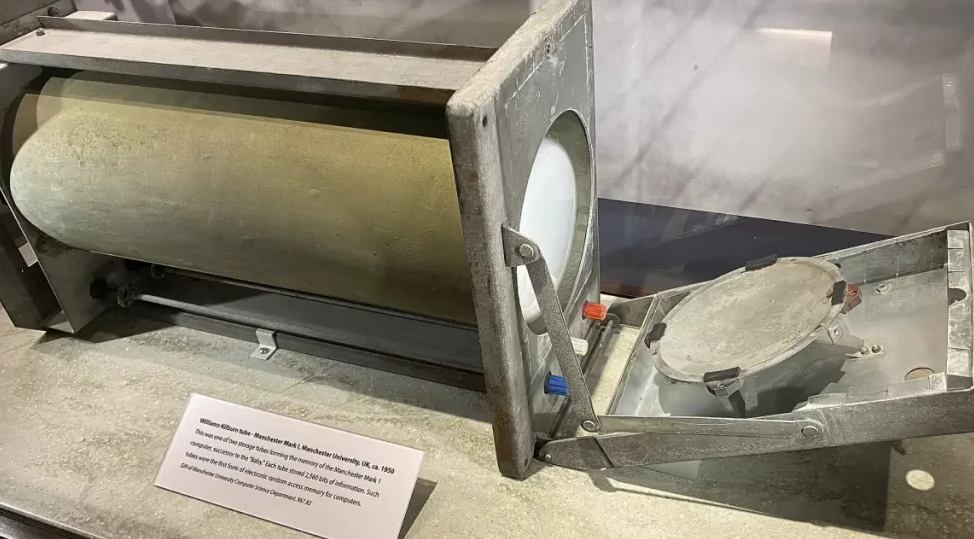
\includegraphics[width=\columnwidth]{media/t02/memoriaTubosWilliams.png}
    \caption{Tubo Williams-Kilburn de almacenamiento electrostático de acceso aleatorio (1947) \parencite[\S 1.2, p.\ 8]{silberschatz2006fundamentos}.}
    \label{fig:memoriaTubosWilliams}
\end{figure}

De forma paralela, entre 1947 y 1949, J. Presper Eckert desarrolló para las computadoras EDVAC y UNIVAC I las líneas de retardo acústico de mercurio (\textit{mercury delay lines}). Este dispositivo electromecánico convertía trenes de impulsos eléctricos en ondas sonoras mecánicas mediante transductores piezoeléctricos de cuarzo situados en los extremos de tubos longitudinales rellenos de mercurio líquido. Las ondas tardaban un intervalo calibrado en viajar a lo largo del medio físico antes de ser reconvertidas en señales eléctricas en el extremo receptor, donde un circuito regenerador las amplificaba y realimentaba al emisor. Si bien este esquema permitía almacenar cientos de bits por columna de mercurio a bajo costo relativo, constituía un almacenamiento secuencial recirculante con tiempos de latencia sumamente elevados y una extrema sensibilidad a las variaciones térmicas que modificaban la velocidad acústica del medio.

La consagración de una memoria principal verdaderamente robusta, compacta y no volátil se alcanzó entre 1949 y 1953 con la invención de la memoria de núcleos magnéticos (\textit{magnetic core memory}), ideada conceptualmente por An Wang y perfectionada arquitectónicamente por Jay Forrester en el proyecto Whirlwind del Instituto Tecnológico de Massachusetts (MIT) e integrada a gran escala por IBM \parencite[\S 2.1, p.\ 32]{mchoes2011sistemas}. Como se aprecia en la Img.~\ref{fig:memoriaNucleosFerrita}, esta memoria se componía de una matriz reticular de pequeños anillos toroidales de ferrita ferromagnética enhebrados en los cruces de conductores de selección coincidentes en los ejes horizontal ($X$) y vertical ($Y$).

\begin{figure}[htbp]
    \centering
    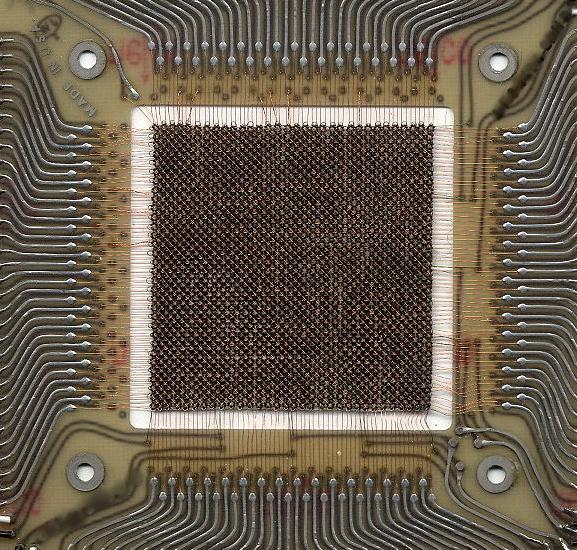
\includegraphics[width=0.6\columnwidth]{media/t02/memoriaNucleosFerrita.jpg}
    \caption{Matriz de memoria de núcleos magnéticos toroidales con hilos de selección coincidentes (1953) \parencite[\S 2.1, p.\ 32]{mchoes2011sistemas}.}
    \label{fig:memoriaNucleosFerrita}
\end{figure}

El principio operativo de los núcleos de ferrita residía en su curva de histéresis magnética rectangular: al aplicar media corriente de conmutación ($\frac{1}{2}I_m$) simultáneamente en una línea $X$ y una línea $Y$, solo el toroide ubicado en la intersección recibía la corriente magnetizante crítica $I_m$ necesaria para invertir su orientación magnética dipolar remanente (en sentido horario o antihorario, codificando el cero o el uno lógico). Al conmutar el estado del núcleo durante la lectura, la variación de flujo magnético inducía una corriente en un hilo sensor común (\textit{sense wire}). Dado que este proceso destruía la orientación previa del bit (lectura destructiva), el controlador requería forzosamente un ciclo complementario de reescritura inmediata asistido por un hilo de inhibición (\textit{inhibit wire}). La memoria de núcleos dominó la industria por más de dos décadas, otorgando al subsistema de memoria principal la denominación histórica de \enquote{núcleo} (core memory) que aún persiste en la terminología técnica \parencite[\S 2.1, p.\ 32]{mchoes2011sistemas}.

El punto de inflexión definitivo hacia el almacenamiento moderno sobre silicio se produjo en 1968, cuando Robert H. Dennard concibió en los laboratorios de IBM la celda de memoria dinámica de un único transistor y un condensador (1T1C). Sobre esta base, en octubre de 1970 la corporación Intel lanzó al mercado el chip Intel 1103, presentado en la Img.~\ref{fig:chipDramIntel1103}. Fabricado con litografía semiconductora de óxido metálico de canal P (PMOS) y encapsulado en una pastilla DIP de 18 pines, el 1103 ofrecía una capacidad de 1024 bits (1 Kibit) a un costo por bit inferior al de los toroides de ferrita, desplazando para siempre a la memoria magnética como estándar de almacenamiento primario e iniciando la era de la memoria dinámica de semiconductores.

\begin{figure}[htbp]
    \centering
    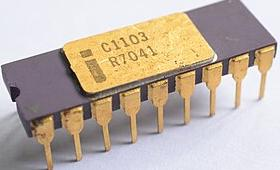
\includegraphics[width=0.6\columnwidth]{media/t02/chipDramIntel1103.jpg}
    \caption{Circuito integrado Intel 1103 en encapsulado DIP de 18 pines, primer chip comercial masivo de memoria DRAM de silicio (1970) \parencite[\S 2.3, p.\ 65]{deitel2004operating}.}
    \label{fig:chipDramIntel1103}
\end{figure}

\subsection{Celdas de memoria de acceso aleatorio: SRAM vs. DRAM}
\label{sec:celdasSramDram}

En la microelectrónica contemporánea coexisten dos arquitecturas fundamentales para la implementación de memorias de lectura y escritura de acceso aleatorio en circuitos integrados: la celda estática (SRAM) y la celda dinámica (DRAM) \parencite[\S 2.3, p.\ 65]{deitel2004operating}. La divergencia entre ambas radica en la física del almacenamiento y en la topología circuital a nivel de transistor:

La celda básica de una memoria \textbf{SRAM} estándar se estructura a partir de seis transistores MOSFET (diseño 6T) formando dos inversores CMOS acoplados en cerrojo biestable (\textit{bistable latch}) gobernado por la línea de palabra (\textit{wordline}) y líneas de bit complementarias (\textit{bitline} y $\overline{\text{\textit{bitline}}}$). Sus propiedades distintivas comprenden: retención continua sin refresco mientras exista alimentación; conmutación ultrarrápida en régimen subnanosegundo (latencias de 0.5 a 3\,ns); y baja densidad con elevado costo por bit, destinándose exclusivamente a las memorias caché multinivel L1--L3 \parencite[\S 2.3, p.\ 65]{deitel2004operating}.

Por su parte, la celda fundamental de una memoria \textbf{DRAM} sigue el diseño minimalista 1T1C de Dennard (un transistor de paso y un condensador de almacenamiento de carga $Q = C \cdot V$). Sus rasgos operativos críticos son: 1) necesidad imperativa de ciclos periódicos de refresco (\textit{refresh cycles}) cada 32 a 64\,ms mediante pulsos automáticos (\textit{auto-refresh}) gobernados por $\overline{\text{RAS}}$ y $\overline{\text{CAS}}$ para compensar fugas subumbral; 2) lectura destructiva restituida por amplificadores de sentido (\textit{sense amplifiers}); y 3) máxima densidad de integración y mínimo costo unitario por gigabyte, erigiéndose en el estándar de memoria principal \parencite[\S 2.3, p.\ 65]{deitel2004operating}.

\subsection{Evolución de las tecnologías DRAM sincrónicas y de alta tasa de transferencia}
\label{sec:evolucionDramSincronica}

Desde la década de 1980, la memoria dinámica evolucionó desde interfaces asíncronas lentas (FPM con retención de línea de fila y EDO con cerrojos de salida para solapar accesos) hacia la estandarización sincrónica por JEDEC con \textbf{SDR SDRAM} (\textit{Single Data Rate Synchronous DRAM}, 1996), alineando comandos y transferencias al reloj del bus (66 a 133\,MHz sobre módulos DIMM de 168 pines) \parencite[\S 2.3, p.\ 65]{deitel2004operating}.

A partir del 2000, la tecnología de doble tasa de transferencia (\textit{Double Data Rate}, DDR) impulsó el ancho de banda efectivo transfiriendo en ambos flancos de reloj y escalando progresivamente los búferes de prebúsqueda: DDR (2000, 2n-prefetch, 2.5\,V, DIMM 184 pines); DDR2 (2003, 4n-prefetch, 1.8\,V, terminación en chip ODT, DIMM 240 pines); DDR3 (2007, 8n-prefetch, 1.5\,V / 1.35\,V); DDR4 (2014, grupos de bancos independientes \textit{Bank Groups}, 1.2\,V, DIMM 288 pines); y DDR5 (2020), que dividió el módulo en dos subcanales de 32 bits, integró administración de potencia PMIC a 1.1\,V, corrección de errores en troquel (\textit{on-die ECC}) y prebúsqueda equivalente 16n (BL16). Especializaciones arquitectónicas abarcan la familia \textbf{LPDDR} (\textit{Low Power DDR}) para dispositivos móviles y memorias apiladas 3D \textbf{HBM} (\textit{High Bandwidth Memory}) con vías pasantes en silicio (TSV) para GPU y aceleradores neuronales.

La Img.~\ref{fig:evolucionModulosDram} ilustra la evolución morfológica de los módulos DIMM estandarizados por JEDEC, y la Tabla~\ref{tab:cronologiaEvolucionRam} sintetiza la cronología integral de la memoria RAM.

\begin{figure}[htbp]
    \centering
    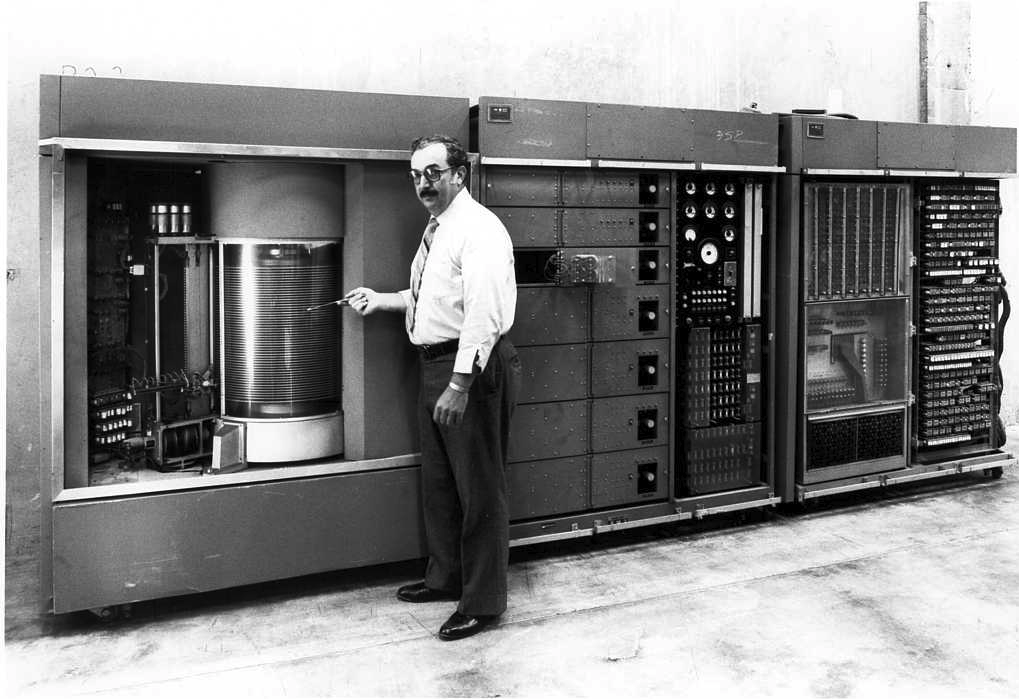
\includegraphics[width=\columnwidth]{media/t02/evolucionModulosDram.png}
    \caption{Comparativa de factores de forma, muescas mecánicas y densidad de pines en módulos DIMM de SDRAM a DDR5 \parencite[\S 2.3, p.\ 65]{deitel2004operating}.}
    \label{fig:evolucionModulosDram}
\end{figure}

\begin{table}[htbp]
\centering
\scriptsize
\renewcommand{\arraystretch}{1.15}
\renewcommand{\tabularxcolumn}[1]{m{#1}}
\setlength{\emergencystretch}{1.5em}
\caption{Cronología evolutiva integral de las tecnologías de memoria principal y RAM.}
\label{tab:cronologiaEvolucionRam}
\begin{tabularx}{\textwidth}{>{\centering\arraybackslash}m{1.2cm} >{\centering\arraybackslash}m{2.2cm} X >{\centering\arraybackslash}m{1.8cm} >{\centering\arraybackslash}m{2.0cm} >{\centering\arraybackslash}m{2.2cm}}
\toprule
\textbf{Año} & \textbf{Denominación} & \textbf{Topología física y celda} & \textbf{Tensión / Pines} & \textbf{Tasa o ancho de banda} & \textbf{Referencia de imagen / Hito} \\
\midrule
1947 & Tubo Williams-Kilburn & Carga electrostática en CRT con emisión secundaria & Alta tensión / Nube analógica & $\approx 1000$ ops/seg \par (1--2 Kb) & Img.~\ref{fig:memoriaTubosWilliams} \par Manchester Baby \\
\addlinespace
1949 & Línea de retardo & Trenes de ondas acústicas en tubos de mercurio & Transductor piezoeléctrico & $\approx 1$ MHz reloj \par Latencia $> 200\,\mu\text{s}$ & EDVAC y UNIVAC I \\
\addlinespace
1953 & Núcleos magnéticos & Toroides de ferrita ferromagnética con selección $X/Y$ & Corriente $I_m$ / Hilos de cobre & Tiempos de ciclo de 1 a 6\,$\mu\text{s}$ & Img.~\ref{fig:memoriaNucleosFerrita} \par MIT Whirlwind / IBM \\
\addlinespace
1970 & Intel 1103 & Circuito integrado DRAM planar de silicio en PMOS & 16 V / DIP 18 pines & Tiempo de acceso de 300\,ns (1 Kb) & Img.~\ref{fig:chipDramIntel1103} \par Primera DRAM comercial \\
\addlinespace
1985 & FPM DRAM & DRAM asíncrona con retención de fila activa ($\overline{\text{RAS}}$) & 5.0 V / SIMM 30--72 pines & Hasta 25 MHz \par Acceso a 60--70\,ns & Sistemas 386 / 486 \\
\addlinespace
1994 & EDO DRAM & Cerrojo de salida para solapamiento de ráfagas $\overline{\text{CAS}}$ & 5.0 V / 3.3 V \par SIMM 72 pines & Hasta 40 MHz \par Acceso a 50\,ns & Pentium clásico \\
\addlinespace
1996 & SDR SDRAM & DRAM sincrónica acoplada al reloj del sistema (JEDEC) & 3.3 V / DIMM 168 pines & 66 a 133 MHz \par 0.53 a 1.06 GB/s & Img.~\ref{fig:evolucionModulosDram} \par PC66, PC100, PC133 \\
\addlinespace
2000 & DDR SDRAM & Doble tasa de datos (subida y bajada), prefetch de 2n & 2.5 V / DIMM 184 pines & 200 a 400 MT/s \par 1.6 a 3.2 GB/s & Módulos DDR-266 / DDR-400 \\
\addlinespace
2003 & DDR2 SDRAM & Prefetch de 4n, bus E/S al doble del núcleo, ODT & 1.8 V / DIMM 240 pines & 400 a 800 MT/s \par 3.2 a 6.4 GB/s & DDR2-667 / DDR2-800 \\
\addlinespace
2007 & DDR3 SDRAM & Prefetch de 8n, bajo voltaje, señalización mejorada & 1.5 V / 1.35 V \par DIMM 240 pines & 800 a 2133 MT/s \par 6.4 a 17.0 GB/s & Módulos DDR3-1600 / DDR3-1866 \\
\addlinespace
2014 & DDR4 SDRAM & Prefetch 8n con Bank Groups, señal POD, conector curvo & 1.2 V / DIMM 288 pines & 1600 a 3200 MT/s \par 12.8 a 25.6 GB/s & DDR4-2400 / DDR4-3200 \\
\addlinespace
2020 & DDR5 SDRAM & Dos subcanales de 32 bits, PMIC en módulo, On-Die ECC & 1.1 V / DIMM 288 pines & 4800 a 8400+ MT/s \par 38.4 a 67.2+ GB/s & DDR5-4800 / DDR5-6000+ \\
\addlinespace
2015+ & HBM / HBM2e & Apilamiento 3D con vías TSV sobre interposer pasivo & 1.2 V / Bus 1024--4096 bits & Hasta 3.2+ Gbps/pin \par $> 1000$ GB/s & Aceleradores GPU e IA \\
\bottomrule
\end{tabularx}
\end{table}

\clearpage

\section{Evolución histórica de la memoria secundaria y almacenamiento masivo}
\label{sec:evolucionMemoriaSecundaria}

\subsection{Tecnologías electromecánicas y magnéticas tempranas}
\label{sec:tecnologiasTempranasAlmacenamiento}

La incapacidad de la memoria principal para retener estados en ausencia de suministro eléctrico ininterrumpido impulsó el desarrollo de subsistemas de almacenamiento secundario persistente masivo \parencite[\S 2.3, p.\ 66]{deitel2004operating}. Los primeros esquemas descansaron en soportes electromecánicos basados en papel perforado, desde la tarjeta perforada de Herman Hollerith (1890) estandarizada por IBM en 1928 (80 columnas de 12 filas rectangulares), sirviendo como medio primario de entrada, salida y resguardo secuencial durante la primera mitad del siglo XX.

La transición hacia medios reescribibles se materializó con la cinta magnética en el subsistema UNISERVO de la computadora UNIVAC I (1951) \parencite[\S 12.1, p.\ 528]{deitel2004operating}. Basada en tiras de mylar con partículas de óxido de hierro ($\text{Fe}_2\text{O}_3$), ofrecía gran capacidad a bajo costo, pero su naturaleza lineal obligaba al rebobinado físico, siendo un acceso estrictamente secuencial que persiste hoy en cartuchos de resguardo terciario LTO (\textit{Linear Tape-Open}) \parencite[\S 1.8, p.\ 21]{silberschatz2006fundamentos}. Para lograr acceso directo sin desplazamiento lineal, Gustav Tauschek concibió en 1932 el tambor magnético (adoptado en la IBM 650 en los años cincuenta), consistente en un cilindro ferromagnético giratorio con cabezales fijos por pista, aunque con capacidad limitada por el área superficial cilíndrica.

La génesis del almacenamiento secundario moderno con acceso aleatorio directo ocurrió el 4 de septiembre de 1956 con el sistema de almacenamiento en disco rígido IBM 305 RAMAC (\textit{Random Access Method of Accounting and Control}) \parencite[\S 12.1, p.\ 528]{deitel2004operating}. Diseñado por el equipo de Reynold B. Johnson, sustituyó el cilindro por un apilamiento vertical de 50 discos de aluminio de 24 pulgadas girando a 1200 RPM, tal como se documenta en la Img.~\ref{fig:discoIbmRamac}.

\begin{figure}[htbp]
    \centering
    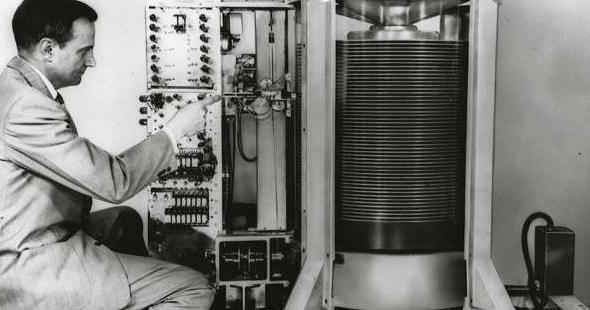
\includegraphics[width=\columnwidth]{media/t02/discoIbmRamac.jpg}
    \caption{Sistema de almacenamiento en disco rígido IBM 305 RAMAC con 50 platos de 24 pulgadas (1956) \parencite[\S 12.1, p.\ 528]{deitel2004operating}.}
    \label{fig:discoIbmRamac}
\end{figure}

Un único brazo gobernado por servoneumáticos se desplazaba verticalmente para seleccionar el plato y radialmente para posicionar el cabezal sobre un cojín de aire a presión. Con una capacidad de 5 millones de caracteres ($\approx 5$\,MB) y una latencia media de 600\,ms, el RAMAC consagró la superioridad del acceso directo y sentó las bases del disco duro moderno \parencite[\S 12.1, p.\ 528]{deitel2004operating}.

\subsection{Medios ópticos y consolidación del disco duro magnético (HDD)}
\label{sec:hddMediosOpticos}

Durante las décadas posteriores al RAMAC, el disco duro magnético (\textit{hard disk drive}, HDD) experimentó una dramática miniaturización e incremento de densidad superficial. En soportes flexibles surgieron los disquetes (\textit{floppy disks}): desarrollados por IBM en 1971 en 8 pulgadas (80\,KB), derivados en 1976 a 5.25 pulgadas (160\,KB a 1.2\,MB) y consolidados por Sony en 1981 en 3.5 pulgadas (1.44\,MB HD en 1987) como estándar universal de intercambio.

La arquitectura del disco duro magnético contemporáneo se consolidó en una estructura mecánica sellada con múltiples platos rígidos a velocidad angular constante (CAV: 5400 a 15000 RPM) \parencites[\S 12.1, pp.\ 409--411]{silberschatz2006fundamentos}[\S 12.3, p.\ 529]{deitel2004operating}, ilustrada en la Img.~\ref{fig:estructuraInternaHdd}.

\begin{figure}[htbp]
    \centering
    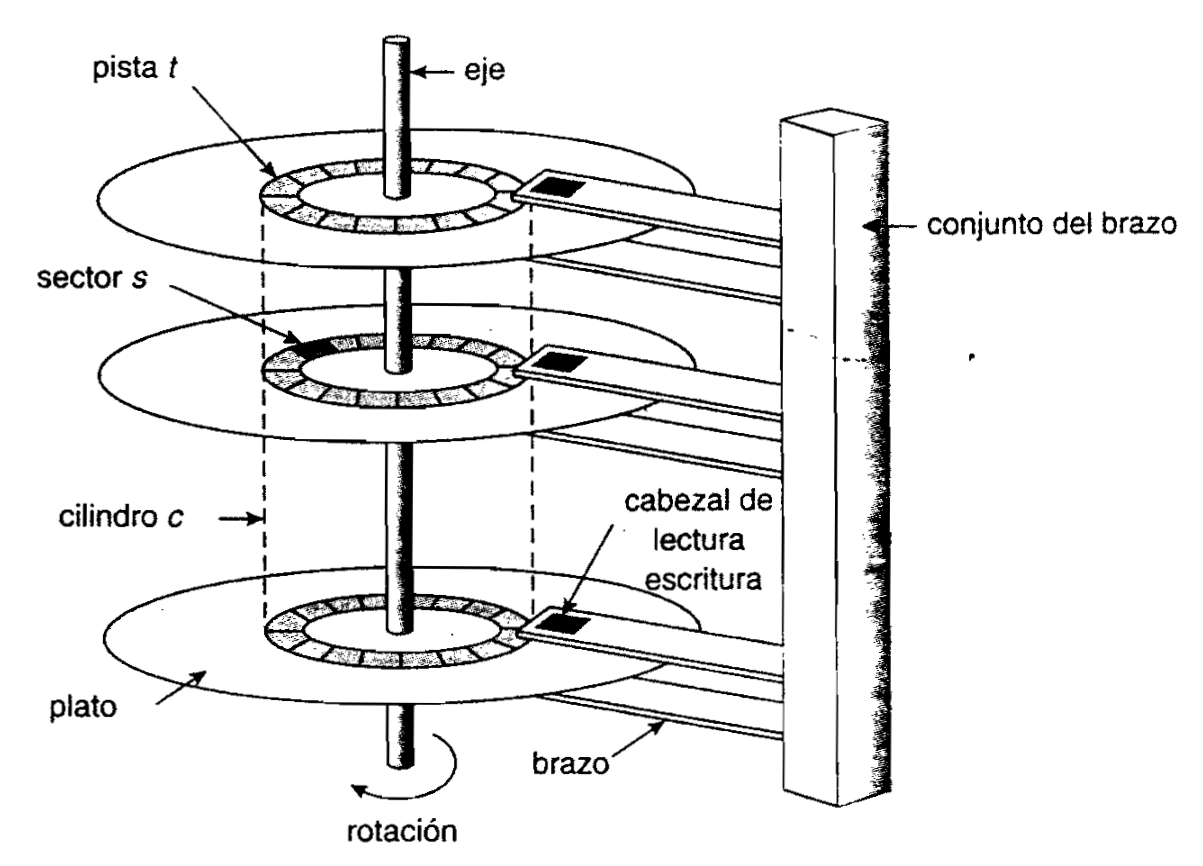
\includegraphics[width=\columnwidth]{media/t02/estructuraInternaHdd.png}
    \caption{Anatomía interna de un disco rígido magnético contemporáneo (platos, cabezales, cilindros y actuador VCM) \parencite[\S 12.1, p.\ 409]{silberschatz2006fundamentos}.}
    \label{fig:estructuraInternaHdd}
\end{figure}

Los cabezales con sensores magnetorresistivos túnel (TMR) vuelan a menos de 10\,nm de la superficie impulsados por un motor de bobina móvil (\textit{voice coil motor}, VCM). La latencia total de acceso responde a tres parámetros temporales \parencite[\S 11.5, pp.\ 518--519]{stallings2018operating}:
\begin{equation}
T_a = T_s + \frac{1}{2r} + \frac{b}{rN}
\label{eq:tiempoAccesoDisco}
\end{equation}
donde $T_s$ es el tiempo medio de búsqueda (*seek time*, 3 a 9\,ms); $\frac{1}{2r}$ es el retardo rotacional medio (*rotational latency*, ej., 4.16\,ms a 7200 RPM); y $\frac{b}{rN}$ es el tiempo de transferencia de $b$ bytes en una pista de $N$ bytes. Lógicamente, el direccionamiento evolucionó de coordenadas físicas CHS a bloques lógicos LBA (\textit{Logical Block Addressing}, sectores de 512B o 4Kn), interconectados mediante SATA III (6 Gbps / AHCI) y SAS (\textit{Serial Attached SCSI}, 12 Gbps), con grabación perpendicular PMR/SMR y sellado con gas helio \parencite[\S 12.2, p.\ 410]{silberschatz2006fundamentos}. En paralelo, surgieron medios ópticos de velocidad lineal constante (CLV) leídos por láser: Compact Disc (CD-ROM, 1982, láser infrarrojo de 780\,nm, 700\,MB), Digital Versatile Disc (DVD, 1995, láser rojo de 650\,nm, 4.7 a 8.5\,GB) y Blu-ray Disc (BD, 2006, láser azul-violeta de 405\,nm, 25 a 100\,GB).

\subsection{Tecnologías de estado sólido y almacenamiento no volátil contemporáneo}
\label{sec:tecnologiasEstadoSolido}

La barrera mecánica de los HDD ($\approx 3$ a 10\,ms) motivó la transición hacia el estado sólido basado en memoria Flash, concebida por Fujio Masuoka en Toshiba (1984 Flash NOR, 1987 Flash NAND) \parencite[\S 12.1, p.\ 528]{deitel2004operating}. La celda Flash NAND almacena carga por tunelamiento cuántico Fowler-Nordheim en compuertas flotantes (\textit{floating-gate}) o trampas de nitruro de silicio (\textit{charge-trap}), alterando la tensión umbral $V_{\text{th}}$ sin requerir energía externa \parencite[\S 1.2, p.\ 9]{silberschatz2006fundamentos}. La densidad escaló por cuantización multinivel: SLC (1 bit/celda), MLC (2 bits), TLC (3 bits) y QLC (4 bits/celda), y por apilamiento tridimensional (3D NAND / V-NAND con más de 200 capas).

Un SSD (\textit{solid-state drive}) moderno integra controlador microprogramado ASIC, DRAM caché y canales Flash paralelos, como se detalla en la Img.~\ref{fig:arquitecturaSsdNvme}.

\begin{figure}[htbp]
    \centering
    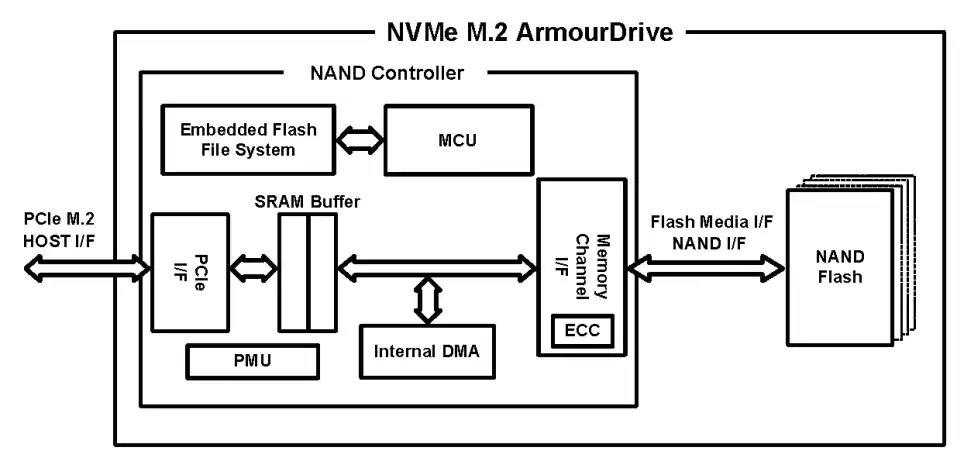
\includegraphics[width=\columnwidth]{media/t02/arquitecturaSsdNvme.png}
    \caption{Diagrama de bloques de un SSD NVMe M.2 con controlador FTL, DRAM y canales Flash 3D NAND \parencite[\S 1.8, p.\ 22]{silberschatz2006fundamentos}.}
    \label{fig:arquitecturaSsdNvme}
\end{figure}

La capa de traducción de Flash (\textit{Flash Translation Layer}, FTL) gestiona la asimetría de la Flash NAND: lectura/escritura por páginas (4--16\,KB) y borrado por bloques completos (2--8\,MB) \parencite[\S 1.2, p.\ 9]{silberschatz2006fundamentos}. Al prohibirse la sobreescritura directa (\textit{no in-place overwrite}), la FTL ejecuta: escritura fuera de lugar con mapeo LBA-PBA; recolección de basura (\textit{garbage collection}) de bloques obsoletos; nivelación de desgaste (\textit{wear leveling}) homogéneo; y procesamiento del comando TRIM / Deallocate del sistema operativo para descartar páginas eliminadas y abatir el factor de amplificación de escritura (WAF). La interfaz NVMe (\textit{Non-Volatile Memory Express}) sobre bus PCIe elimina cuellos de botella con hasta 64\,000 colas paralelas de 64\,000 comandos cada una \parencite[\S 1.8, p.\ 22]{silberschatz2006fundamentos}. La Tabla~\ref{tab:cronologiaMemoriaSecundaria} resume la cronología evolutiva del almacenamiento secundario.

En interconexión, los primeros SSD adoptaron SATA III con protocolo AHCI, que concebido para discos magnéticos rotatorios limitaba transferencias a una cola de 32 comandos y 600 MB/s. La superación de este cuello de botella provino del protocolo NVMe (\textit{Non-Volatile Memory Express}), diseñado para operar sobre el bus PCI Express (PCIe 3.0, 4.0 y 5.0). NVMe reemplaza la cola única de AHCI con una arquitectura escalable de hasta 64,000 colas con 64,000 comandos cada una, reduciendo sustancialmente ciclos de CPU por E/S y elevando transferencias secuenciales a 7,000--14,000 MB/s en factores compactos M.2 y U.2/EDSFF, con latencias de 10 a 20 microsegundos.

Finalmente, en el extremo más avanzado de la jerarquía no volátil emergieron memorias de cambio de fase como 3D XPoint (comercializada como Intel Optane), basada en una matriz de cruce de conductores (\textit{cross-point}) sin transistores que conmutaba la resistencia de un material calcogenuro. Al brindar direccionamiento por byte y lecturas/escrituras simétricas sin requerir ciclos de borrado de bloque, 3D XPoint operaba como memoria de clase almacenamiento (\textit{storage-class memory}, SCM), cerrando la brecha de rendimiento entre la DRAM y la memoria Flash NAND.

La Tabla~\ref{tab:cronologiaMemoriaSecundaria} detalla la cronología evolutiva integral de las tecnologías de memoria secundaria y almacenamiento masivo.

\begin{table}[htbp]
\centering
\scriptsize
\renewcommand{\arraystretch}{1.15}
\renewcommand{\tabularxcolumn}[1]{m{#1}}
\setlength{\emergencystretch}{1.5em}
\caption{Cronología evolutiva integral de las tecnologías de memoria secundaria y almacenamiento.}
\label{tab:cronologiaMemoriaSecundaria}
\begin{tabularx}{\textwidth}{>{\centering\arraybackslash}m{1.2cm} >{\centering\arraybackslash}m{2.2cm} X >{\centering\arraybackslash}m{1.8cm} >{\centering\arraybackslash}m{2.0cm} >{\centering\arraybackslash}m{2.2cm}}
\toprule
\textbf{Año} & \textbf{Tecnología y denominación} & \textbf{Soporte físico y mecanismo} & \textbf{Capacidad / Factor de forma} & \textbf{Latencia / Velocidad típica} & \textbf{Hito o referencia de imagen} \\
\midrule
1890 & Tarjetas perforadas & Cartulina con perforaciones físicas en matriz & 80 columnas \par $\approx 80$ bytes/tarjeta & Lectura mecánica \par $100$--$1000$ tarj/min & Herman Hollerith \par IBM censo 1890 \\
\addlinespace
1951 & Cinta magnética & Película de mylar con recubrimiento de óxido de hierro & Carrete $1/2''$ \par 1.4 MB por cinta & Acceso secuencial \par $100$ bytes/pulgada & UNIVAC I \par UNISERVO \\
\addlinespace
1953 & Tambor magnético & Cilindro metálico giratorio con cabezales fijos por pista & Cilindros dedicados \par 10 a 60 KB & Retardo rotacional \par $\approx 10$ a $20\,\text{ms}$ & IBM 650 mainframe \\
\addlinespace
1956 & IBM 305 RAMAC & 50 platos de aluminio de 24 pulgadas y cabezal neumático & 5 MB (7 bits) \par Mueble masivo & Latencia $\approx 600\,\text{ms}$ \par 8.8 KB/s & Img.~\ref{fig:discoIbmRamac} \par Primer HDD comercial \\
\addlinespace
1971 & Disquete (Floppy) & Disco flexible de mylar protegido en funda de plástico & 8'', 5.25'', 3.5'' \par 80 KB a 1.44 MB & Rotación a 300 RPM \par Latencia $> 100\,\text{ms}$ & IBM 3740 y Sony \par Almacenamiento portátil \\
\addlinespace
1980 & HDD 5.25'' / 3.5'' & Platos rígidos en rotación CAV y actuador de bobina VCM & ST-506, IDE/PATA \par 5 MB a 500 MB & Seek time de 15--40\,ms \par Transferencia $< 5$ MB/s & Seagate ST-506 \par Estandarización de PC \\
\addlinespace
1982 & CD-ROM & Lectura óptica de pozos/planos con láser infrarrojo (780 nm) & Disco de 120 mm \par 650 a 700 MB & Modo CLV 1x \par 150 KB/s ($1200\,\mu\text{s}$) & Estándar Red/Yellow Book \par Philips / Sony \\
\addlinespace
1995 & DVD-ROM & Pistas ópticas estrechas leídas por haz láser rojo (650 nm) & Disco de 120 mm \par 4.7 GB a 8.5 GB & Modo CLV 1x \par 1.38 MB/s ($150\,\mu\text{s}$) & Consorcio DVD \par Video y software masivo \\
\addlinespace
2000+ & HDD SATA / SAS & Platos con grabación PMR/SMR y cavidad de helio & 3.5'' / 2.5'' \par 1 TB a 24+ TB & Seek time de 4--8\,ms \par 150 a 280 MB/s & Img.~\ref{fig:estructuraInternaHdd} \par Almacenamiento masivo \\
\addlinespace
2006 & Blu-ray Disc & Láser azul-violeta (405 nm) de alta apertura numérica & Disco de 120 mm \par 25 GB a 100 GB & Modo CLV 1x \par 4.5 MB/s (hasta 54 MB/s) & Distribución HD y BDXL \\
\addlinespace
2008 & SSD SATA (NAND) & Matrices Flash NAND con FTL sobre bus SATA III AHCI & Factor de forma 2.5'' \par 64 GB a 4 TB & Latencia $\approx 100\,\mu\text{s}$ \par Máximo 550 MB/s & Adopción de estado sólido \\
\addlinespace
2015 & SSD NVMe PCIe & Flash 3D NAND vertical sobre bus PCIe con colas paralelas & Factor M.2 / U.2 \par 500 GB a 8+ TB & Latencia 10--20\,$\mu\text{s}$ \par 3500 a 14000 MB/s & Img.~\ref{fig:arquitecturaSsdNvme} \par PCIe 3.0 / 4.0 / 5.0 \\
\addlinespace
2015 & 3D XPoint & Memoria de cambio de fase resistiva sin borrado de bloque & M.2 / Add-In Card \par 16 GB a 1.5 TB & Latencia $< 10\,\mu\text{s}$ \par Ultra alta durabilidad & Intel Optane / Micron \par Storage-Class Memory \\
\bottomrule
\end{tabularx}
\end{table}

\clearpage

\section{Memoria de intercambio (Swapping) y gestión de memoria virtual}

\subsection{Definición y distinción técnica: intercambio de procesos frente a paginación bajo demanda}

En la ingeniería de sistemas operativos, la memoria de intercambio (\textit{swapping}) es el mecanismo mediante el cual el núcleo transfiere temporalmente regiones del espacio de direccionamiento desde la memoria física primaria (DRAM) hacia un almacén de respaldo (\textit{backing store}) secundario, liberando marcos físicos y restituyendo la información al reanudarse la tarea \parencite[\S 8.2, p.\ 249]{silberschatz2006fundamentos}. Arquitectónicamente, debe distinguirse entre el \textbf{intercambio clásico} de procesos (\textit{roll out / roll in}) en particiones continuas, donde el kernel trasladaba en bloque la imagen íntegra del proceso (código, datos, montón y pila) con severas penalizaciones temporales de E/S que elevaban el costo del cambio de contexto a niveles prohibitivos \parencite[\S 7.2, p.\ 343]{stallings2018operating}, y la \textbf{paginación bajo demanda} (\textit{demand paging}) asistida por la MMU contemporánea, donde el intercambio opera a nivel de páginas virtuales de 4 KB \parencite[\S 4.6, p.\ 165]{carretero2001sistemas}, cargadas bajo fallo de página (\textit{page fault}) y desalojadas selectivamente a disco (\textit{page-out}) sin transferir estructuras completas \parencite[\S 9.2, p.\ 283]{silberschatz2006fundamentos}.

El subsistema clasifica las páginas según su origen de respaldo: las \textit{páginas respaldadas por archivos} (\textit{file-backed}), como código ejecutable o bibliotecas compartidas, que al ser desalojadas no requieren escribirse al swap si permanecen limpias (\textit{clean}), pues se recargan del binario original; y la \textit{memoria anónima} (\textit{anonymous memory}), integrada por la pila (\textit{stack}), montón (\textit{heap}) y variables modificadas, que al carecer de respaldo persistente deben escribirse obligatoriamente en el área de intercambio para evitar la pérdida del estado de cómputo \parencite[\S 12.4, p.\ 415]{silberschatz2006fundamentos}.

\subsection{Funciones y operatividad de la memoria de intercambio en el sistema operativo}

La memoria de intercambio cumple tres funciones operativas cardinales en el núcleo \parencite[\S 8.1, p.\ 371]{stallings2018operating}: 1) \textbf{Ampliación del espacio de direccionamiento}, proyectando una memoria virtual global superior a la DRAM física para admitir cargas analíticas pesadas \parencite[\S 10.3, p.\ 432]{deitel2004operating}; 2) \textbf{Regulación de la multiprogramación}, permitiendo suspender procesos dormidos o bloqueados en E/S prolongada y enviar sus páginas inactivas a disco para hacer espacio a tareas listas \parencite[\S 3.2, p.\ 136]{stallings2018operating}; y 3) \textbf{Optimización de la caché de páginas (\textit{page cache})}, donde el kernel expulsa páginas anónimas infrecuentes para ceder marcos libres a la caché de archivos, acelerando la E/S global del sistema \parencite[\S 4.9, p.\ 181]{carretero2001sistemas}.

Estructuralmente, el área de intercambio opera como una \textit{partición dedicada} (\textit{swap partition}) sin sobrecarga de inodos mediante mapa de ranuras (\textit{swap map}), o como un \textit{archivo de intercambio} (\textit{swap file}, ej., \texttt{pagefile.sys} o montajes vía \texttt{swapon}) de redimensionamiento dinámico \parencite[\S 12.4, p.\ 416]{silberschatz2006fundamentos}. Cada ranura (\textit{swap slot}) equivale a una página física y mantiene contadores de referencia para páginas compartidas (\textit{copy-on-write}) \parencite[\S 9.3, p.\ 289]{silberschatz2006fundamentos}. El desalojo es modulado por la sobreasignación (\textit{memory overcommit}) y la afinidad (\textit{swappiness}), que balancea de 0 a 100 el rescate de páginas de caché frente al swap anónimo.

\subsection{Rendimiento, degradación por hiperpaginación (\textit{Thrashing}) y mecanismos de mitigación}

La hiperpaginación (thrashing) ocurre cuando el conjunto agregado de procesos activos no dispone de marcos físicos suficientes para mantener sus páginas de uso frecuente, provocando una cascada continua de fallos de página \parencite[\S 9.6.1, p.\ 305]{silberschatz2006fundamentos}. En este estado, los procesos seleccionados por la CPU detienen su ejecución esperando lecturas de swap; el despachador interpreta la subutilización de CPU como baja carga e introduce más procesos, colapsando el bus de E/S y reduciendo el rendimiento útil a cero \parencite[\S 8.2, p.\ 388]{stallings2018operating}.

Para erradicar la hiperpaginación, Peter J. Denning formuló en 1968 el modelo del conjunto de trabajo (\textit{working set model}) basado en el principio de localidad \parencite[\S 9.6.2, p.\ 307]{silberschatz2006fundamentos}. Definiendo una ventana temporal de referencias recientes $\Delta$, el conjunto de trabajo $W_i(t, \Delta)$ contiene las páginas virtuales referenciadas por el proceso $i$ en $[t - \Delta, t]$. La demanda total de marcos corresponde a:
\begin{equation}
    D = \sum_{i=1}^{n} |W_i(t, \Delta)|
\end{equation}
donde $|W_i(t, \Delta)|$ es la cardinalidad de páginas activas del proceso $i$. La estabilidad exige que la demanda no exceda los marcos físicos disponibles ($D \le M$); si $D > M$, el planificador debe suspender y expulsar procesos completos a disco hasta restaurar el balance \parencite[\S 8.2, p.\ 401]{stallings2018operating}. Complementariamente, la política de frecuencia de fallos de página (\textit{page-fault frequency}, PFF) asigna o confisca marcos monitoreando umbrales dinámicos $\tau_{\text{inf}}$ y $\tau_{\text{sup}}$ \parencite[\S 9.6.3, p.\ 308]{silberschatz2006fundamentos}. Ante agotamiento crítico, mecanismos como el Asesino de Fuera de Memoria (\textit{Out-Of-Memory Killer}, OOM Killer) calculan una función de nocividad (\textit{badness score}) para terminar forzosamente mediante \texttt{SIGKILL} el proceso más gravoso, preservando la estabilidad del núcleo \parencite[\S 11.6, p.\ 494]{deitel2004operating}.

\clearpage

\section{Arquitectura y ciclo de vida de los procesos}

\subsection{Definición formal de proceso y organización en memoria}

En la teoría de sistemas operativos, un proceso se define formalmente como un programa en ejecución, constituyendo la entidad activa fundamental de cómputo y la unidad elemental de asignación de recursos protegidos del procesador \parencite[\S 3.1.1, p.\ 73]{silberschatz2006fundamentos}. Esta definición establece una demarcación rigurosa frente al concepto de programa: mientras que un programa es una entidad estática y pasiva almacenada en soporte no volátil como una secuencia binaria estructurada bajo formatos como ELF (\textit{Executable and Linkable Format}) o PE (\textit{Portable Executable}), un proceso es una entidad dinámica caracterizada por un hilo de control, un espacio virtual exclusivo, estados de ejecución cambiantes y posesión activa de recursos del sistema \parencite[\S 3.1, p.\ 131]{stallings2018operating}.

El espacio de direccionamiento virtual asignado a un proceso por el núcleo se descompone en cinco regiones o segmentos contiguos en memoria lógica \parencite[\S 3.3.2, p.\ 103]{carretero2001sistemas}: 1) \textbf{Segmento de texto (\textit{text segment})}, con instrucciones de máquina en direcciones bajas con permisos de sólo lectura y ejecución, dotado de reentrancia para compartir marcos físicos; 2) \textbf{Segmento de datos inicializados (\textit{data segment})}, reservado para variables globales y estáticas con valor inicial explícito; 3) \textbf{Segmento de datos no inicializados (\textit{Block Started by Symbol}, BSS)}, para variables globales sin inicializar, asignadas a cero por el cargador del kernel sin ocupar espacio en disco \parencite[\S 3.3.2, p.\ 104]{carretero2001sistemas}; 4) \textbf{Montón (heap)}, zona de asignación dinámica solicitada por llamadas como \texttt{brk} o \texttt{malloc}, cuyo límite crece hacia direcciones altas \parencite[\S 3.1.1, p.\ 74]{silberschatz2006fundamentos}; y 5) \textbf{Pila de llamadas (call stack)}, estructura LIFO en direcciones superiores que desciende hacia el montón, almacenando marcos de activación con parámetros, retornos y variables locales \parencite[\S 3.3, p.\ 151]{stallings2018operating}. Una franja intermedia no mapeada previene colisiones accidentales entre pila y montón.

\subsection{Estructura y características del proceso: Bloque de Control de Proceso (PCB)}

El comportamiento operativo del proceso exhibe cuatro características cardinales \parencite[\S 3.1, p.\ 97]{carretero2001sistemas}: 1) \textbf{Concurrencia}, permitiendo intercalar su ejecución con otros flujos en el procesador; 2) \textbf{Asincronía y no determinismo}, dado que su progreso depende de latencias de E/S y decisiones del planificador; 3) \textbf{Aislamiento y protección espacial}, garantizados por la MMU mediante tablas de páginas independientes que prohíben accesos ilícitos ajenos \parencite[\S 3.1, p.\ 132]{stallings2018operating}; y 4) \textbf{Posesión de recursos}, fungiendo como titular de descriptores de archivos, memoria y cuotas de cómputo.

Para gobernar estos recursos, el sistema materializa cada proceso mediante el Bloque de Control de Proceso (\textit{Process Control Block}, PCB; \texttt{task\_struct} en Linux) \parencite[\S 3.1.3, p.\ 75]{silberschatz2006fundamentos}, estructurado en cinco áreas clave \parencite[\S 3.3, p.\ 152]{stallings2018operating}: 1) \textbf{Identificación}, con identificador de proceso (PID), del padre (PPID) y credenciales UID/GID; 2) \textbf{Contexto de hardware}, con contador de programa (PC), puntero de pila (SP), registros generales, banderas y registro de tabla de páginas (CR3 en x86) para conmutación \parencite[\S 3.1.3, p.\ 76]{silberschatz2006fundamentos}; 3) \textbf{Planificación}, con estado y colas del despachador; 4) \textbf{Memoria}, con descriptores virtuales y tablas de páginas (\texttt{mm\_struct}); y 5) \textbf{Contabilidad y E/S}, con descriptores de archivos, dispositivos y consumo de CPU.

\subsection{Modelo de estados y transiciones en la ejecución del proceso}

El ciclo vital de un proceso transita por estados discretos formalizados por el modelo clásico de cinco estados \parencite[\S 3.2, p.\ 133]{stallings2018operating}: \textbf{Nuevo (\textit{New})}, durante la inicialización del PCB y asignación preliminar de descriptores \parencite[\S 3.1.2, p.\ 74]{silberschatz2006fundamentos}; \textbf{Listo (\textit{Ready})}, con todas las páginas residentes en memoria física esperando turno de CPU; \textbf{En ejecución (\textit{Running})}, con instrucciones ejecutándose activamente en los registros del procesador; \textbf{Bloqueado (\textit{Blocked})}, aguardando la finalización de una operación de E/S o un evento de sincronización \parencite[\S 3.5, p.\ 115]{carretero2001sistemas}; y \textbf{Terminado (\textit{Exit})}, concluido mediante la llamada \texttt{exit}, reteniendo su PCB en estado zombi (\textit{zombie}) hasta que el padre recolecta su código de terminación mediante \texttt{wait} \parencite[\S 3.3.2, p.\ 85]{silberschatz2006fundamentos}.

La dinámica de ejecución se articula mediante transiciones gobernadas por el planificador del kernel \parencite[\S 3.2, p.\ 134]{stallings2018operating}: 1) \textit{Admisión} (Nuevo $\to$ Listo), cuando el sistema valida la disponibilidad de memoria; 2) \textit{Despacho} (Listo $\to$ Ejecución), al asignar el procesador según la política de turnos; 3) \textit{Expropiación o fin de cuanto} (Ejecución $\to$ Listo), gatillada por la interrupción periódica del reloj del sistema (*timer interrupt*) en esquemas apropiativos; 4) \textit{Bloqueo} (Ejecución $\to$ Bloqueado), cuando el proceso emite una llamada al sistema bloqueante; y 5) \textit{Despertar} (Bloqueado $\to$ Listo), originado por una interrupción de hardware que notifica la disponibilidad del periférico.

Ante saturación severa de memoria física y riesgo de hiperpaginación, Stallings formula el \textit{modelo de siete estados}, integrando el almacenamiento secundario con dos estados de suspensión \parencite[\S 3.2, p.\ 138]{stallings2018operating}: \textbf{Listo-suspendido (\textit{Ready/Suspend})}, el cual se encuentra en condiciones de ejecutar pero reside temporalmente en el área de swap; y \textbf{Bloqueado-suspendido (\textit{Blocked/Suspend})}, que aguarda un evento de E/S mientras su imagen permanece desalojada a disco. Este modelo introduce la optimización de \textit{resolución de evento en swap}: al concluir la operación de E/S externa, el controlador del dispositivo promueve el proceso directamente desde Bloqueado-suspendido hacia Listo-suspendido sin forzar la recarga inmediata de sus marcos a la DRAM, permitiendo al planificador de mediano plazo evaluar estratégicamente el momento óptimo de reinserción según la carga global del sistema \parencite[\S 3.2, p.\ 140]{stallings2018operating}.

\clearpage

\section{Hilos de ejecución y análisis comparativo frente a procesos}

\subsection{Definición formal de hilo (\textit{Thread}) y estructura de control (TCB)}

En la ingeniería de sistemas operativos, un hilo de ejecución (thread, hebra o proceso ligero) se define formalmente como la unidad elemental de despacho y utilización de la CPU, constituyendo un flujo secuencial independiente dentro del espacio de un proceso \parencite[\S 4.1, p.\ 111]{silberschatz2006fundamentos}. Esta conceptualización formaliza una dualidad arquitectónica: el proceso representa la unidad de \textbf{propiedad de recursos} y protección espacial, mientras que el hilo constituye la unidad de \textbf{planificación y ejecución temporal} \parencite[\S 4.1, p.\ 177]{stallings2018operating}.

Los hilos de un proceso comparten homogéneamente su espacio virtual (texto, datos, BSS y montón), descriptores de archivos, sockets y manejadores de señales \parencite[\S 4.1, p.\ 112]{silberschatz2006fundamentos}. Cada hilo preserva autonomía mediante elementos privados exclusivos: identificador de hilo (TID), contexto volátil de registros (PC, SP y registros generales), pila de llamadas propia (\textit{per-thread stack}) y almacenamiento local (TLS). El núcleo materializa esta entidad mediante el Bloque de Control de Hilo (\textit{Thread Control Block}, TCB) \parencite[\S 3.6, p.\ 121]{carretero2001sistemas}; en Linux, la gestión converge en \texttt{task\_struct} mediante la llamada \texttt{clone()} con banderas de compartición (\texttt{CLONE\_VM}, \texttt{CLONE\_FILES}, \texttt{CLONE\_SIGHAND}) \parencite[\S 4.6, p.\ 208]{stallings2018operating}.

\subsection{Modelos de gestión de hilos y correspondencia de planificación}

La administración de hilos se bifurca según el nivel arquitectónico que gestiona su ciclo de vida \parencite[\S 4.2, p.\ 183]{stallings2018operating}: los \textbf{hilos a nivel de usuario} (\textit{User-Level Threads}, ULT), coordinados por bibliotecas en espacio de usuario sin intervención del kernel, ofrecen conmutación rápida sin cambio de modo de privilegio (\textit{mode switch}), pero carecen de paralelismo multinúcleo y bloquean al proceso completo ante una llamada al sistema síncrona; y los \textbf{hilos a nivel de núcleo} (\textit{Kernel-Level Threads}, KLT), despachados por el planificador del kernel, que habilitan ejecución paralela simétrica y tolerancia a bloqueos de E/S a cambio de una mayor sobrecarga de transición al modo supervisor \parencite[\S 4.2, p.\ 187]{stallings2018operating}. La correspondencia entre ambas capas se articula mediante tres modelos \parencite[\S 4.2, pp.\ 114--117]{silberschatz2006fundamentos}: \textbf{Muchos a uno ($N:1$)}, con múltiples ULT sobre un único KLT; \textbf{Uno a uno ($1:1$)}, estándar de facto en Linux (NPTL) y Windows que asocia cada ULT a un KLT dedicado; y \textbf{Muchos a muchos ($M:N$)}, que multiplexa dinámicamente $M$ hilos de usuario sobre $N$ hilos de núcleo ($M \ge N$).

\clearpage

\subsection{Estudio comparativo y diferencial entre procesos e hilos}

El contraste entre procesos pesados e hilos abarca dimensiones críticas de desempeño, arquitectura y diseño de software \parencite[\S 4.1, p.\ 179]{stallings2018operating}. En el ámbito de la instanciación, crear un proceso mediante la llamada al sistema \texttt{fork()} impone una sobrecarga notable: el núcleo debe duplicar o mapear estructuras de tablas de páginas, reservar descriptores de archivos, asignar un nuevo espacio de direcciones virtuales y configurar cuotas de planificación, requiriendo típicamente entre 10 y 30 veces más ciclos de procesador que instanciar un hilo mediante \texttt{pthread\_create()}, el cual únicamente exige reservar la estructura TCB y asignar una pila privada en el montón del proceso \parencite[\S 4.1, p.\ 179]{stallings2018operating}.

En la conmutación de contexto, alternar la CPU entre procesos distintos exige invalidar o actualizar los registros del búfer de traducción anticipada (TLB) y modificar el registro de control de la tabla de páginas (como el registro CR3 en la arquitectura x86), provocando una degradación temporal del rendimiento por fallos de caché fríos. En contraparte, conmutar entre hilos del mismo proceso preserva íntegramente las traducciones de la memoria virtual activa en el TLB y las líneas de caché de datos e instrucciones, reduciendo la penalización al simple guardado y restauración de los registros de trabajo del procesador y del puntero de pila \parencite[\S 3.5.1, p.\ 119]{carretero2001sistemas}.

En el paradigma de comunicación interna, los procesos demandan mecanismos formales de comunicación entre procesos (IPC) como tuberías (*pipes*), colas de mensajes, memoria compartida (\texttt{shmget}) o sockets de red locales, requiriendo validaciones de seguridad por el kernel y copias intermedias de búferes \parencite[\S 3.4, pp.\ 86--90]{silberschatz2006fundamentos}. Por el contrario, los hilos se comunican de forma instantánea leyendo y modificando variables globales y estructuras en el montón común. No obstante, esta accesibilidad introduce el riesgo de condiciones de carrera (\textit{race conditions}), forzando al programador a incorporar primitivas explícitas de sincronización (cerrojos de exclusión mutua *mutex*, semáforos contadores de Dijkstra y variables de condición) sustentadas en instrucciones atómicas del procesador como *Compare-And-Swap* (CAS) \parencite[\S 4.1, p.\ 112]{silberschatz2006fundamentos}.

Finalmente, en cuanto a tolerancia a fallos y seguridad, el proceso provee una barrera de aislamiento infranqueable garantizada por la MMU: una excepción fatal o fallo de segmentación (\texttt{SIGSEGV}) queda confinado estrictamente a su contexto. En cambio, al carecer de aislamiento de memoria entre sí, un puntero erróneo o violación de acceso en un único hilo desencadena el colapso inmediato e integral de todo el proceso contenedor. La Tabla~\ref{tab:comparativaProcesosHilos} sintetiza de forma estructurada las divergencias operativas y arquitectónicas entre ambos esquemas.

\clearpage

\begin{table}[htbp]
\centering
\scriptsize
\renewcommand{\arraystretch}{1.06}
\renewcommand{\tabularxcolumn}[1]{m{#1}}
\setlength{\emergencystretch}{1.5em}
\caption{Estudio comparativo y diferencial entre procesos pesados e hilos de ejecución.}
\label{tab:comparativaProcesosHilos}
\begin{tabularx}{\textwidth}{>{\centering\arraybackslash}m{2.5cm} X X}
\toprule
\textbf{Criterio diferencial} & \textbf{Proceso (Proceso pesado)} & \textbf{Hilo de ejecución (Proceso ligero)} \\
\midrule
\textbf{Rol arquitectónico} & Unidad formal de posesión de recursos, contabilidad y protección espacial \parencite[\S 4.1, p.\ 177]{stallings2018operating}. & Unidad elemental de despacho de procesador, planificación y flujo de ejecución \parencite[\S 4.1, p.\ 111]{silberschatz2006fundamentos}. \\
\addlinespace[2pt]
\textbf{Espacio de memoria} & Espacio de direcciones virtuales privado e independiente, aislado por tablas de la MMU. & Comparte el espacio virtual del proceso contenedor (texto, datos, BSS, montón) con pila propia. \\
\addlinespace[2pt]
\textbf{Estructura de control} & Bloque de Control de Proceso (PCB / \texttt{task\_struct}), con descriptores y mapa de memoria. & Bloque de Control de Hilo (TCB), limitado a identificador (TID), registros volátiles, PC y SP. \\
\addlinespace[2pt]
\textbf{Sobrecarga de creación} & Elevada: exige replicar o mapear estructuras de páginas, descriptores de archivos y cuotas de cómputo. & Mínima: requiere únicamente reservar el TCB y una pila privada (10 a 30 veces más rápida) \parencite[\S 4.1, p.\ 179]{stallings2018operating}. \\
\addlinespace[2pt]
\textbf{Cambio de contexto} & Penalización temporal alta: requiere invalidar el búfer TLB y conmutar el registro CR3 de la tabla de páginas. & Conmutación liviana: preserva las entradas del TLB y la tabla de páginas activa; sólo conmuta registros y SP \parencite[\S 3.5.1, p.\ 119]{carretero2001sistemas}. \\
\addlinespace[2pt]
\textbf{Comunicación interna} & Exige mecanismos de IPC (tuberías, colas de mensajes, memoria compartida \texttt{shmget}, sockets de red). & Comunicación directa por variables globales en el montón; exige cerrojos mutex y semáforos \parencite[\S 4.1, p.\ 112]{silberschatz2006fundamentos}. \\
\addlinespace[2pt]
\textbf{Aislamiento y fallos} & Protección espacial total: una excepción fatal o fallo de segmentación queda confinado al proceso. & Sin aislamiento de memoria: un puntero erróneo o violación de acceso en un hilo aborta el proceso íntegro. \\
\bottomrule
\end{tabularx}
\end{table}

\clearpage

\section{Conclusiones personales}

El estudio sistemático de la memoria y la gestión de procesos demuestra que el diseño de los sistemas operativos descansa en una continua mediación entre abstracciones de software y restricciones del hardware. La jerarquía de memoria surge como una respuesta imperativa a la brecha insalvable entre la velocidad de la CPU y las latencias de almacenamiento. Desde tecnologías pioneras como los tubos Williams y núcleos de ferrita magnética hasta la consolidación de la DRAM y los discos NVMe de estado sólido, cada avance ha mitigado el cuello de botella de von Neumann. En este esquema, la unidad de manejo de memoria (MMU) y la virtualización del direccionamiento constituyen los pilares que otorgan a cada tarea la ilusión de disponer de un espacio contiguo, uniforme y protegido contra interferencias externas.

Por su parte, la memoria de intercambio (swapping) y la paginación bajo demanda evidencian que la memoria física no limita de forma estricta el grado de multiprogramación. Al trasladar selectivamente páginas inactivas y memoria anónima hacia el disco, el núcleo maximiza el aprovechamiento de la memoria principal y optimiza la memoria caché de archivos. Sin embargo, este balance es delicado: la hiperpaginación (thrashing) ejemplifica cómo una sobreasignación de memoria o un deficiente seguimiento del conjunto de trabajo anulan el ancho de banda útil del procesador. El empleo de mecanismos adaptativos como la política de frecuencia de fallos de página y salvaguardas de última instancia como el OOM Killer subraya el rigor matemático necesario para prevenir la degradación catastrófica del sistema.

Finalmente, la dualidad entre procesos e hilos consolida los paradigmas modernos de concurrencia. Mientras el proceso proporciona una frontera infranqueable de aislamiento espacial, posesión de recursos y contabilidad protegida por hardware, el hilo aporta la agilidad requerida para explotar procesadores multinúcleo mediante conmutaciones de contexto livianas y memoria compartida. Como futuros ingenieros en computación, dominar estos conceptos es crucial, pues la elección entre la robustez del aislamiento por procesos y la eficiencia cooperativa de los hilos determina directamente la estabilidad, el desempeño y la escalabilidad de cualquier plataforma computacional.

\nocite{*}
\printbibliography[heading=bibintoc, title={Referencias}]

\end{document}
